
\section{Data Preparation}
\label{sec:background}

The following data preparation and preprocessing steps were completed independently and identically in both the red wine and white wine data sets. All experimental methodologies and data manipulation was completed using auxiliary Python libraries including \textit{scikit-learn}, \textit{numpy}, \textit{pandas}, and \textit{matplotlib}. The data was first shuffled, and one-fifth of it was held out for a final testing set. The remaining 80\% of the data was used for training our regression models. \\\\
We plotted individual features against the wine quality to visualize if there were any apparent relationships between them (seen below). As we expected, this varied depending on which feature was chosen. Some features in the red wine dataset, such as alcohol and volatile acidity, showed a directional preference as wine quality increased. This indicated that indeed, some features appear to correlate with a higher quality wine. For others, such as residual sugar, there was no obvious correlation between the feature and the wine quality. \\\\
\begin{figure}[htb]

  \centering  % centers the image in the column

  % replace the second argument below with your filename. I like to
  % place all my figures in a sub-directory to keep things organized
  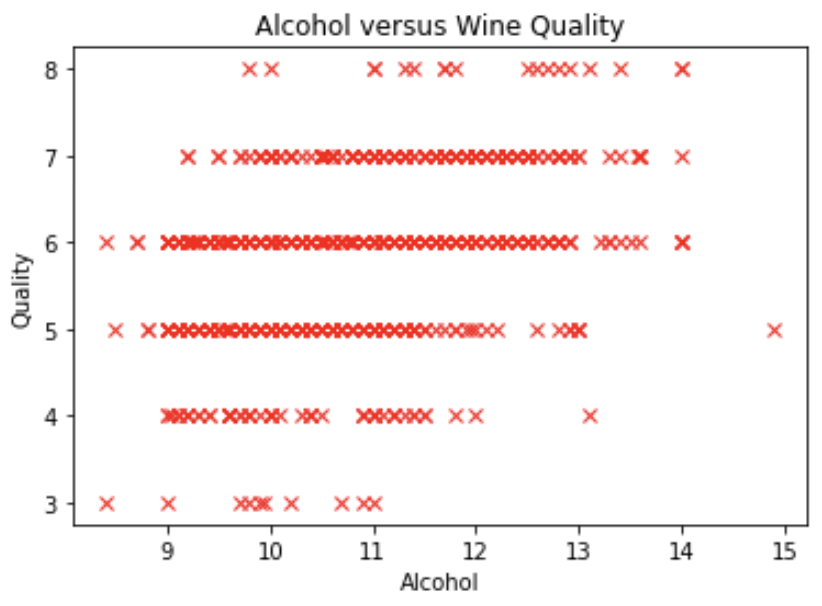
\includegraphics[width=\linewidth]{template/figs/alcohol.png}

  % *Every* figure should have a descriptive caption.
  \caption{This distribution of wine qualities and their alcohol content indicates a slight positive correlation between the two variables.}

  % The label is a handle you create so that you can refer to this
  % figure (using the \ref{} command) from other parts of your
  % document. LaTeX automatically renumbers figures and updates
  % references when you recompile, so you should do it this way rather
  % than hard-coding in references. Notice that I've also been
  % creating labels for the various sections in the document; I could
  % use \ref{} command to refer to those sections using their labels
  % too.
  \label{fig:alcohol}

\end{figure}

\begin{figure}[htb]

  \centering  % centers the image in the column

  % replace the second argument below with your filename. I like to
  % place all my figures in a sub-directory to keep things organized
  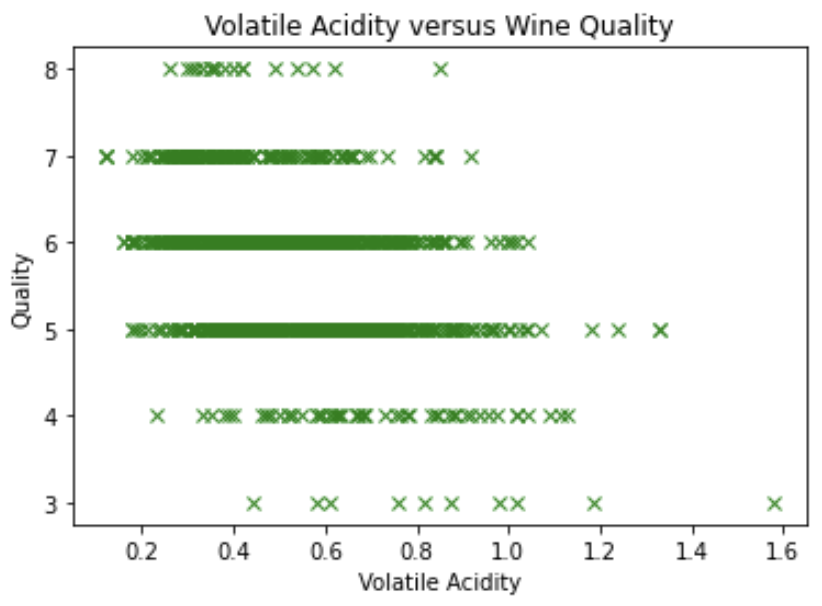
\includegraphics[width=\linewidth]{template/figs/acidity.png}

  % *Every* figure should have a descriptive caption.
  \caption{This distribution of wine qualities and their volatile acidity indicates a slight negative correlation between the two variables.}

  % The label is a handle you create so that you can refer to this
  % figure (using the \ref{} command) from other parts of your
  % document. LaTeX automatically renumbers figures and updates
  % references when you recompile, so you should do it this way rather
  % than hard-coding in references. Notice that I've also been
  % creating labels for the various sections in the document; I could
  % use \ref{} command to refer to those sections using their labels
  % too.
  \label{fig:acidity}

\end{figure}

\begin{figure}[htb]

  \centering  % centers the image in the column

  % replace the second argument below with your filename. I like to
  % place all my figures in a sub-directory to keep things organized
  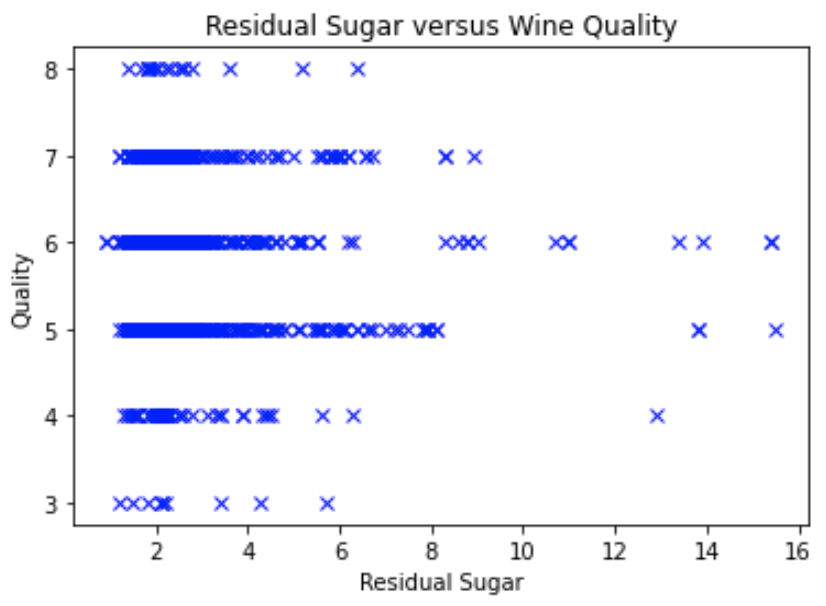
\includegraphics[width=\linewidth]{template/figs/sugar.png}

  % *Every* figure should have a descriptive caption.
  \caption{There is no strong correlation between wine quality and residual sugar.}

  % The label is a handle you create so that you can refer to this
  % figure (using the \ref{} command) from other parts of your
  % document. LaTeX automatically renumbers figures and updates
  % references when you recompile, so you should do it this way rather
  % than hard-coding in references. Notice that I've also been
  % creating labels for the various sections in the document; I could
  % use \ref{} command to refer to those sections using their labels
  % too.
  \label{fig:sugar}

\end{figure}
This exploratory phase of our experiment was crucial to the implementation of our solution. These findings indicated some features might be more correlated than others, and led us to consider using a specific type of regression which focuses on reducing the impact of unrelated variables on our model. \\\\
The eleven input features of the dataset were then scaled using standardization. This transforms the data into a normal distribution feature-wise, which will allow the regression solver to more efficiently converge on a solution. More on this can be found in Scikit-Learn’s data preprocessing user guide \cite{sklearn_api}. \\\\
With all of this background information, we made several key choices with our regression models that allow for the more efficient and accurate prediction model. \\\\